\documentclass[12pt,a4paper]{article}
\usepackage[utf8]{inputenc}
\usepackage[T1]{fontenc}
\usepackage{amsmath}
\usepackage{textcomp}

\usepackage{geometry}
\geometry{a4paper,left=25mm,right=25mm, top=2cm, bottom=2cm} 

\usepackage{graphicx} %fuer bilder

\usepackage{verbatim}



 \usepackage{mathptmx}
 \usepackage[scaled=.90]{helvet}
 \usepackage{courier}


\usepackage{listings}
\usepackage{color}
 
\definecolor{dkgreen}{rgb}{0,0.6,0}
\definecolor{gray}{rgb}{0.5,0.5,0.5}
\definecolor{mauve}{rgb}{0.58,0,0.82}

\pagestyle{empty}
\lstset{numbers=left,language=C++}
\lstset{showstringspaces=false,
basicstyle=\ttfamily\footnotesize,
breaklines=true,
tabsize=3,
commentstyle=\color{dkgreen},      % comment style
inputencoding={ansinew},
title=\lstname %zeigt titel der datei an
}

\usepackage{pdfpages}% fuer pdfs



%keine einrückungen bei absatz
\parindent 0pt

\begin{document}
\title{Übung 02}
\author{Bernhard Selymes; Reinhard Penn}
\date{April 2013}

\normalsize

%Pfad zu c++ Dateien


%Beginn des Dokuments

\newcommand{\Uebung}{Uebung02}
\newcommand{\path}{../Uebung02}

%Angabe
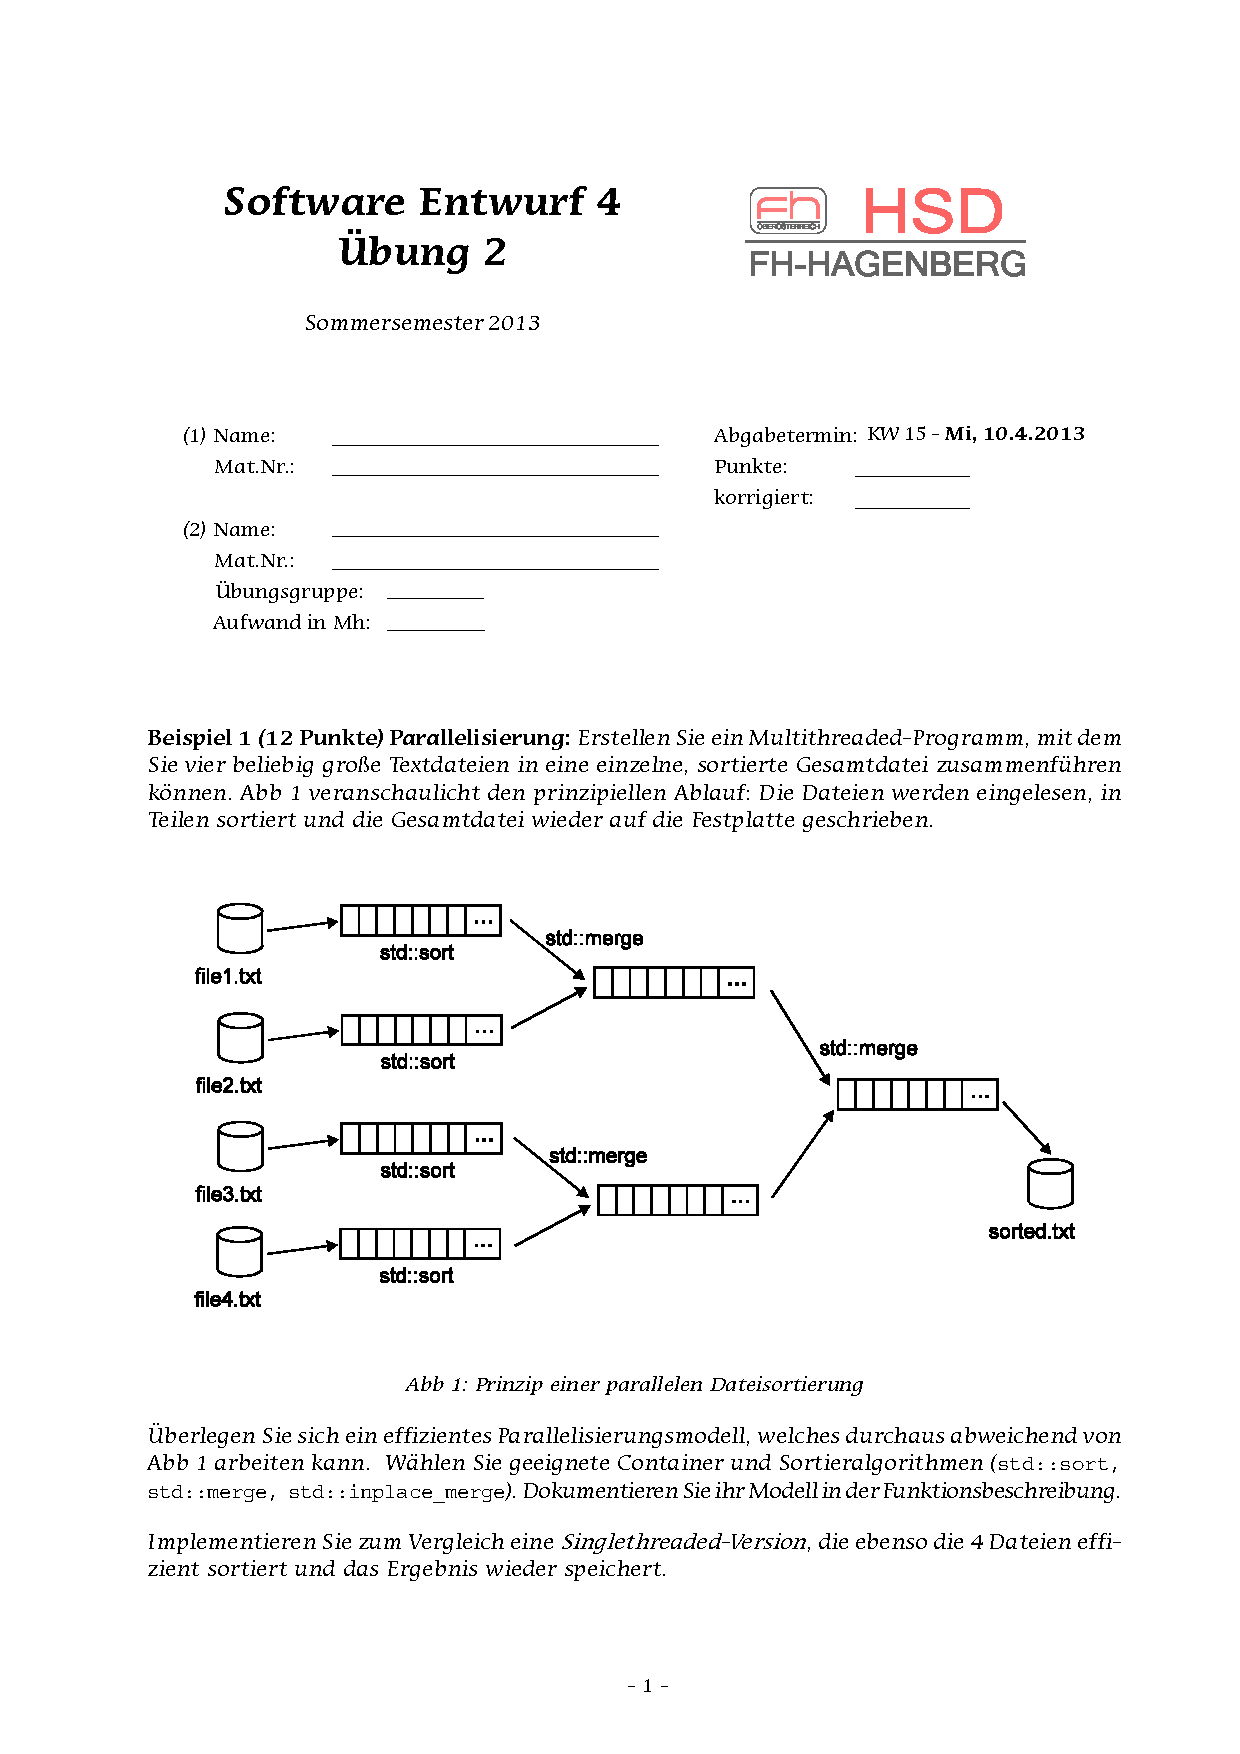
\includepdf[pages=-]{../Angabe.pdf}

\section{Beispiel 1}
\subsection{Funktionsbeschreibung}

Es gibt 4 verschiedene Arten von Workerthreads: 
\begin{itemize}
\item Datei zu Liste
\item Liste zu Datei
\item Liste sortieren
\item 2 Listen zusammenfügen
\end{itemize}
Es gibt für jede Arbeit einen eigenen Thread, dadurch ist die Software übersichtlicher und leichter erweiterbar. Zum Beispiel beliebige Anzahl von Eingangsdateien oder auch Ausgangsdateien. Der Thread der die letzte Liste in die Datei schreibt hätte auch wie die singlethreaded Version implementiert werden können und wäre dadurch auch schneller gewesen. Im Mainthread werden die Handles in Vektoren verwaltet. Von dort werden sie den Threads gegeben. Die Threads warten auf die Threads von denen sie die Handles haben und schließen diese danach.
\newline
Die Daten der Dateien werden in 4 Listen gespeichert. Diese 4 Listen werden sortiert. Danach werden 2 mal 2 Listen zusammengefügt und wieder danach werden die letzten 2 Listen zusammengefügt. Die letzte Liste wird wieder in die Datei geschrieben.
\newline
Anmerkung: Es wurden keine Fehlerfälle im Testtreiber getestet, weil diese  durch Exceptions abgefangen werden würden.
\newline 
Aufgabenaufteilung: Beispiel 1: Bernhard Selymes, Beispiel 2: Reinhard Penn

\subsection{Schnittstellen}
Name: SortMergeMT(...) und SortMergeST(...)
\newline
Parameter: vector<string> const\& filenames, string const\& filenameOutput
\newline
Vektor wegen Erweiterbarkeit und einfacherer Handhabung.
\newline
\newline
\textbf{Schnittstellen der Threads:} Bei der Init Funktion werden jeweils die benötigten Listen und Handles mitgegeben. Die Listen via Pointer, weil sonst die ganze Liste kopiert werden müsste und auch die falsche Liste verändert werden würde. Diese Parameter werden in den Threads jeweils gespeichert.

\subsection{Singlethreaded Version}
Bei dieser Version werden die Daten aller Dateien gleich in eine Liste geschrieben. Diese Liste wird dann sortiert und wieder in eine Datei geschrieben.
\newline
\textbf{Speedup:} 
\newline
Speedup  = 5.885/5.695 = 1.0334
\newline
Die längste Zeit dauert das Schreiben auf die Festplatte.

\newpage
\subsection{Sourcecode}
\lstinputlisting[language={c++}]{\path/Bsp01/StopWatch.h}
\lstinputlisting[language={c++}]{\path/Bsp01/StopWatch.cpp}

\lstinputlisting[language={c++}]{\path/Bsp01/ThreadBase.h}
\lstinputlisting[language={c++}]{\path/Bsp01/ThreadBase.cpp}

\lstinputlisting[language={c++}]{\path/Bsp01/ThreadFileToList.h}
\lstinputlisting[language={c++}]{\path/Bsp01/ThreadFileToList.cpp}

\lstinputlisting[language={c++}]{\path/Bsp01/ThreadListToFile.h}
\lstinputlisting[language={c++}]{\path/Bsp01/ThreadListToFile.cpp}

\lstinputlisting[language={c++}]{\path/Bsp01/ThreadSort.h}
\lstinputlisting[language={c++}]{\path/Bsp01/ThreadSort.cpp}

\lstinputlisting[language={c++}]{\path/Bsp01/ThreadMerge.h}
\lstinputlisting[language={c++}]{\path/Bsp01/ThreadMerge.cpp}

\lstinputlisting[language={c++}]{\path/Bsp01/SortMergeMT.h}
\lstinputlisting[language={c++}]{\path/Bsp01/SortMergeMT.cpp}

\lstinputlisting[language={c++}]{\path/Bsp01/main.cpp}

\lstinputlisting[language={c++}]{\path/Bsp01_SingleThreaded/SortMergeST.h}
\lstinputlisting[language={c++}]{\path/Bsp01_SingleThreaded/SortMergeST.cpp}

\lstinputlisting[language={c++}]{\path/Bsp01_SingleThreaded/main.cpp}

\newpage
\subsection{Testausgabe}
Multithreaded(Release):
\begin {verbatim}
Start timer.
End timer. Time: 5.695
Press a key...
\end {verbatim}

Multithreaded(Debug ohne Ende(dauert ewig)):
\begin {verbatim}
Start timer.
Error in SortMergeMT::SortMergeMT: no valid vector
Error in SortMergeMT::SortMergeMT: no valid string at index 0
Error in SortMergeMT::SortMergeMT: no valid vector
Error in SortMergeMT::SortMergeMT: no valid filenameOutput
\end {verbatim}

Singlethreaded(Release):
\begin {verbatim}
Start timer.
End timer. Time: 5.885
Press a key...
\end {verbatim}

Singlethreaded(Debug ohne Ende(dauert ewig)):
\begin {verbatim}
Start timer.
Error in SortMergeST::SortMergeST: no valid vector
Error in SortMergeST::SortMergeST: no valid string at index 0
Error in SortMergeST::SortMergeST: no valid vector
Error in SortMergeST::SortMergeST: no valid filenameOutput
\end {verbatim}

\newpage
\section{Beispiel 2}

\subsection{Funktionsbeschreibung}

%\newline
%\newline
%\textbf{Schnittstelle:}
%\newline
%Name: CreateThreadsFib
%\newline
%Returnwert: void
%\newline
%Parameter: 
%\newline
%size\_t num: Anzahl der zu erstellenden Threads
%\newline
%size\_t fibMax: Grenzwert der Fibonacci Berechnungen


\subsection{Sourcecode}
%\lstinputlisting[language={c++}]{\path/MainThreadWorkerThread/Fibonacci.h}
%\lstinputlisting[language={c++}]{\path/MainThreadWorkerThread/Fibonacci.cpp}
%\newpage
%\lstinputlisting[language={c++}]{\path/MainThreadWorkerThread/MainThreadWorkerThread.h}
%\lstinputlisting[language={c++}]{\path/MainThreadWorkerThread/MainThreadWorkerThread.cpp}
%\newpage
%\lstinputlisting[language={c++}]{\path/MainThreadWorkerThread/main.cpp}

\subsection{Testausgabe}

\begin{verbatim}

\end{verbatim}


\end{document}
